\documentclass{article}

\newif\ifanswers
\answerstrue % comment out to hide answers

\usepackage[compact]{titlesec}
\usepackage{fancyhdr} % Required for custom headers
\usepackage{lastpage} % Required to determine the last page for the footer
\usepackage{extramarks} % Required for headers and footers
\usepackage[usenames,dvipsnames]{color} % Required for custom colors
\usepackage{graphicx} % Required to insert images
\usepackage{listings} % Required for insertion of code
\usepackage{courier} % Required for the courier font
\usepackage{lipsum} % Used for inserting dummy 'Lorem ipsum' text into the template
\usepackage{enumerate}
\usepackage{enumitem}
\usepackage{subfigure}
\usepackage{booktabs}
\usepackage{amsmath, amsthm, amssymb}
\usepackage[maxbibnames=99,maxcitenames=1]{biblatex}
\usepackage{caption}
\usepackage{hyperref}
\captionsetup[table]{skip=4pt}
\usepackage{framed}
\usepackage{bm}
\usepackage{minted}
\usepackage{soul}
\usepackage[utf8]{vietnam}
\usepackage[vietnamese,english]{babel}

\graphicspath{{images/}}

\addbibresource{references.bib} %Import the bibliography file
\AtNextBibliography{\small}

\usepackage{tikz}
\usetikzlibrary{positioning, patterns, fit}


% Margins
\topmargin=-0.45in
\evensidemargin=0in
\oddsidemargin=0in
\textwidth=6.5in
\textheight=9.0in
\headsep=0.25in

\linespread{1.1} % Line spacing

% Set up the header and footer
\pagestyle{fancy}
\rhead{\hmwkAuthorName} % Top left header
\lhead{\hmwkClass: \hmwkTitle} % Top center head
\lfoot{\lastxmark} % Bottom left footer
\cfoot{} % Bottom center footer
\rfoot{Page\ \thepage\ of\ \protect\pageref{LastPage}} % Bottom right footer
\renewcommand\headrulewidth{0.4pt} % Size of the header rule
\renewcommand\footrulewidth{0.4pt} % Size of the footer rule

\setlength\parindent{0pt} % Removes all indentation from paragraphs

\newenvironment{answer}{
    % Uncomment this if using the template to write out your solutions.
    {\bf Answer:} \sf \begingroup\color{red}
}{\endgroup}%
%----------------------------------------------------------------------------------------
%	CODE INCLUSION CONFIGURATION
%----------------------------------------------------------------------------------------

\definecolor{MyDarkGreen}{rgb}{0.0,0.4,0.0} % This is the color used for comments
\definecolor{shadecolor}{gray}{0.9}

\lstloadlanguages{Python} % Load Perl syntax for listings, for a list of other languages supported see: ftp://ftp.tex.ac.uk/tex-archive/macros/latex/contrib/listings/listings.pdf
\lstset{language=Python, % Use Perl in this example
        frame=single, % Single frame around code
        basicstyle=\footnotesize\ttfamily, % Use small true type font
        keywordstyle=[1]\color{Blue}\bf, % Perl functions bold and blue
        keywordstyle=[2]\color{Purple}, % Perl function arguments purple
        keywordstyle=[3]\color{Blue}\underbar, % Custom functions underlined and blue
        identifierstyle=, % Nothing special about identifiers
        commentstyle=\usefont{T1}{pcr}{m}{sl}\color{MyDarkGreen}\small, % Comments small dark green courier font
        stringstyle=\color{Purple}, % Strings are purple
        showstringspaces=false, % Don't put marks in string spaces
        tabsize=5, % 5 spaces per tab
        %
        % Put standard Perl functions not included in the default language here
        morekeywords={rand},
        %
        % Put Perl function parameters here
        morekeywords=[2]{on, off, interp},
        %
        % Put user-defined functions here
        morekeywords=[3]{test},
       	%
        morecomment=[l][\color{Blue}]{...}, % Line continuation (...) like blue comment
        numbers=left, % Line numbers on left
        firstnumber=1, % Line numbers start with line 1
        numberstyle=\tiny\color{Blue}, % Line numbers are blue and small
        stepnumber=5 % Line numbers go in steps of 5
}

% Creates a new command to include a perl script, the first parameter is the filename of the script (without .pl), the second parameter is the caption
\newcommand{\perlscript}[2]{
\begin{itemize}
\item[]\lstinputlisting[caption=#2,label=#1]{#1.pl}
\end{itemize}
}

%----------------------------------------------------------------------------------------
%	NAME AND CLASS SECTION
%----------------------------------------------------------------------------------------

\newcommand{\hmwkTitle}{Homework 2} % Assignment title
\newcommand{\hmwkClass}{INT3404E 20 - Image Processing} % Course/class
\newcommand{\hmwkAuthorName}{Trần Phương Linh} % Your name

\newcommand{\ifans}[1]{\ifanswers \color{red} \vspace{5mm} \textbf{Solution: } #1 \color{black} \vspace{5mm} \fi}

% Chris' notes
\definecolor{CMpurple}{rgb}{0.6,0.18,0.64}
\newcommand\cm[1]{\textcolor{CMpurple}{\small\textsf{\bfseries CM\@: #1}}}
\newcommand\cmm[1]{\marginpar{\small\raggedright\textcolor{CMpurple}{\textsf{\bfseries CM\@: #1}}}}

%----------------------------------------------------------------------------------------
%	TITLE PAGE
%----------------------------------------------------------------------------------------
\title{
\vspace{-1in}
\textmd{\textbf{\hmwkClass:\ \hmwkTitle} \\ \hmwkAuthorName}\\
}
\author{}
% \date{\textit{\small Updated \today\ at \currenttime}} % Insert date here if you want it to appear below your name
\date{}

\setcounter{section}{0} % one-indexing
\begin{document}
\maketitle

\section{Ex1 - Image Filtering}
\subsection{Source code}
\subsubsection{padding\_img() function}
\begin{lstlisting}[caption={Code of padding\_img() function}, label={padding\_img}]
def padding_img(img, filter_size=3):
    pad_size = filter_size // 2
    padded_img = np.pad(img, pad_size, mode='edge')
    return padded_img
\end{lstlisting}

\begin{itemize}
    
    \item Algorithm:
    \begin{itemize}
        \item Use the np.pad function from the NumPy library to add rows and columns around the original image. The pad\_size parameter is calculated by dividing filter\_size by 2, and then np.pad is used to add the corresponding rows and columns.
        \item The mode is set to 'edge', which means that the pixel values at the edges of the image will be copied from the last rows and columns of the image. This helps preserve the edges of the image and avoid creating unwanted effects when padding.
    \end{itemize}
\end{itemize}


\subsubsection{mean\_filter() function}
\begin{lstlisting}[caption={Code of mean\_filter() function}, label={mean\_filter()}]
def mean_filter(img, filter_size=3):
    # Perform padding
    padded_img = padding_img(img, filter_size)

    # Get image shape
    height, width = img.shape

    # Initialize smoothed image
    smoothed_img = np.zeros_like(img)

    # Apply mean filter
    for i in range(height):
        for j in range(width):
            # Extract neighborhood
            neighborhood = padded_img[i:i + filter_size, j:j + filter_size]
            # Apply mean filter
            smoothed_img[i, j] = np.mean(neighborhood)

    return smoothed_img
\end{lstlisting}

\begin{itemize}
    
    \item Algorithm:
    \begin{itemize}
        \item The input image is padded using the padding\_img function, ensuring pixels at the edge of the image can also be processed.
        \item A matrix with the same size as the input image is initialized to contain the smoothed image.
        \item The function goes through each pixel of the image, and at each location, extracts the neighborhood around that pixel using the filter size.

        \item The median filter is applied by calculating the average of the pixel values in the neighborhood.
        \item The mean value is assigned to the corresponding pixel in the smoothed image.
   
    \end{itemize}
\end{itemize}



\subsubsection{median\_filter() function}
\begin{lstlisting}[caption={Code of median\_filter() function}, label={median\_filter()}]
def median_filter(img, filter_size=3):
    # Perform padding
    padded_img = padding_img(img, filter_size)

    # Get image shape
    height, width = img.shape

    # Initialize smoothed image
    smoothed_img = np.zeros_like(img)

    # Apply median filter
    for i in range(height):
        for j in range(width):
            # Extract neighborhood
            neighborhood = padded_img[i:i + filter_size, j:j + filter_size]
            # Apply median filter
            smoothed_img[i, j] = np.median(neighborhood)

    return smoothed_img
\end{lstlisting}

\begin{itemize}
    
    \item Algorithm:
    \begin{itemize}
        \item The input image is padded using the padding\_img function, ensuring pixels at the edge of the image can also be processed.
        \item A matrix with the same size as the input image is initialized to contain the smoothed image.
        \item The function goes through each pixel of the image, and at each location, extracts the neighborhood around that pixel using the filter size.
        \item The median filter is applied by calculating the median of the pixel values in the neighborhood.
        \item The median value is assigned to the corresponding pixel in the smoothed image.
    \end{itemize}
\end{itemize}


\subsubsection{psnr() function}
\begin{lstlisting}[caption={Code of psnr() function}, label={psnr()}]
def psnr(gt_img, smooth_img):
    # Calculate Mean Square Error (MSE)
    mse = np.mean((gt_img - smooth_img) ** 2)

    # Maximum possible pixel value
    max_pixel = 255

    # Calculate PSNR
    psnr_score = 10 * math.log10((max_pixel ** 2) / mse)

    return psnr_score
\end{lstlisting}

\begin{itemize}
    
    \item Algorithm:
    \begin{itemize}
        \item Calculate the MSE (Mean Square Error) value between the original image and the filtered image, then use the given PSNR formula to calculate the PSNR score and return it.
    \end{itemize}
\end{itemize}



\subsection{Output}
\subsubsection{Results after performing the mean filter}
\begin{itemize}
    \item Image after performing the mean filter:
\end{itemize}

\begin{figure}[H]
    \centering
    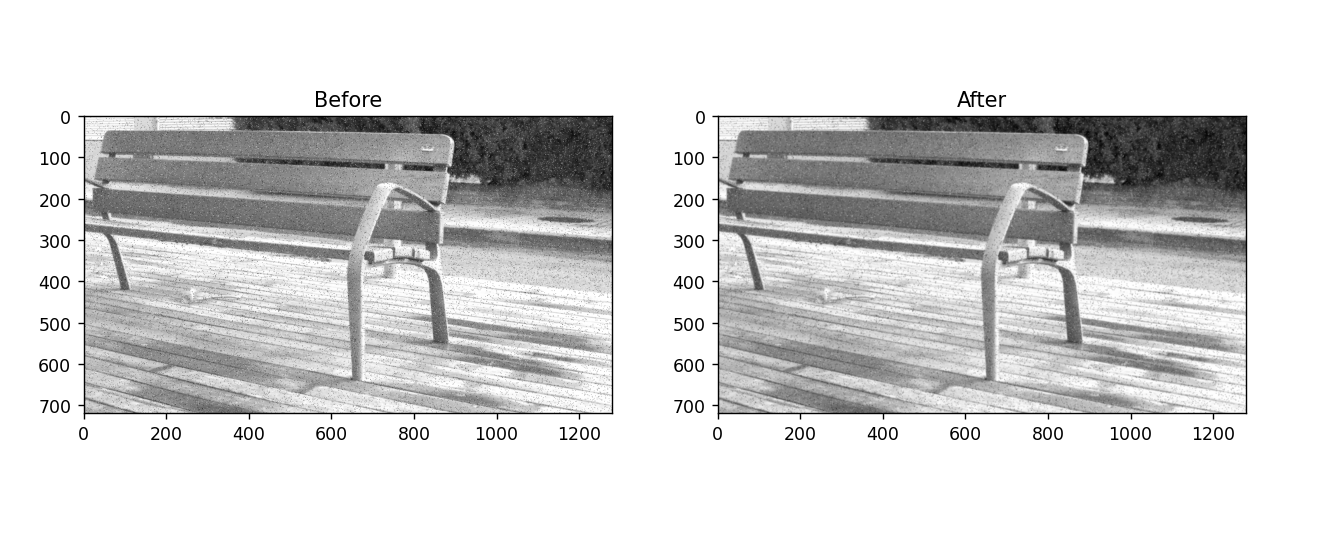
\includegraphics[width=0.75\textwidth]{before-after-mean}
    \caption{After mean filter}
    \label{before-after-mean}
\end{figure}

\begin{itemize}
    \item PSNR score value: \lstinline{31.61}
\end{itemize}

\subsubsection{Results after performing the median filter}
\begin{itemize}
    \item Image after implementing the median filter:
\end{itemize}

\begin{figure}[H]
    \centering
    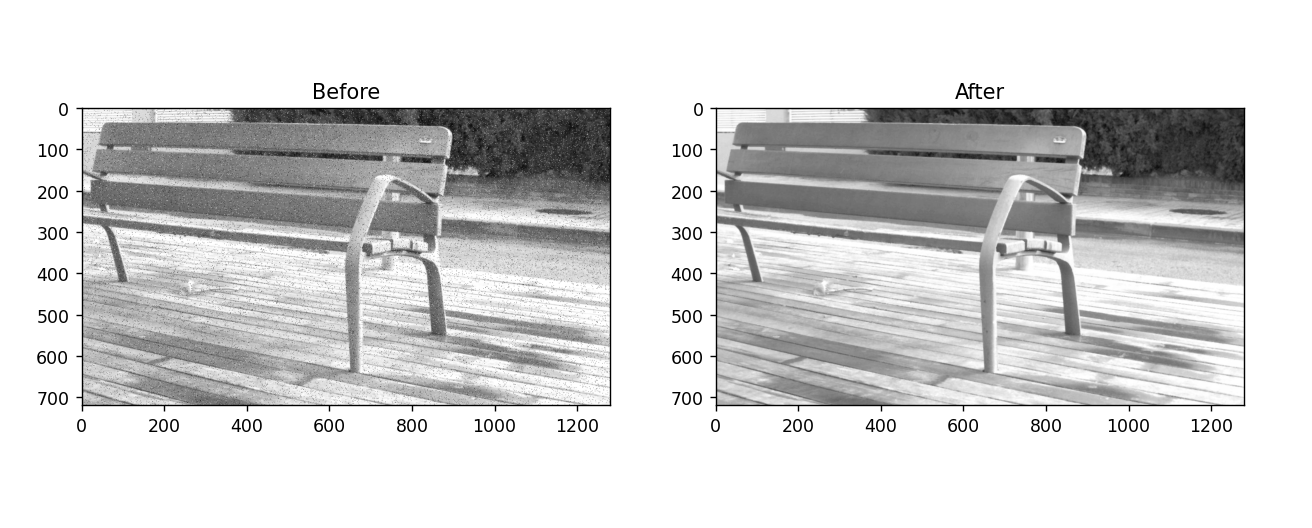
\includegraphics[width=0.75\textwidth]{before-after-median}
    \caption{After median filter}
    \label{before-after-median}
\end{figure}

\begin{itemize}
    \item PSNR score value: \lstinline{37.12}
\end{itemize}

\subsubsection{Comments on PSNR score}

\begin{itemize}
    \item Based on the provided Peak Signal-to-Noise Ratio (PSNR) metrics:
    \begin{itemize}
        \item Mean filter PSNR score: 31.61
        \item Median filter PSNR score: 37.12
    \end{itemize}
    
    \item The PSNR score measures the quality of an image after filtering, where a higher PSNR value indicates better image quality. In this case, the median filter has a significantly higher PSNR score than the mean filter. This implies that the median filter has better performance in preserving image quality and reducing noise.
    \item Therefore, considering the PSNR metrics, median filter should be chosen over mean filter for the provided images.
    
\end{itemize}



\section{Ex 2.1 và Ex 2.2 - Fourier Transform}
\subsection{Source code}

\subsubsection{DFT\_slow() function}
\begin{lstlisting}[caption={Code of DFT\_slow() function}]
def DFT_slow(data):
    N = len(data)
    n = np.arange(N)
    k = n.reshape((N, 1))
    e = np.exp(-2j * np.pi * k * n / N)
    return np.dot(e, data)
\end{lstlisting}

\begin{itemize}
    \item Source code:
    \begin{itemize}
        \item Determines the length of the input data.
        \item Create a numpy array containing indices from 0 to data length - 1.
        \item Create a matrix of exponents.
        \item Compute the DFT by multiplying the exponents matrix with the input data and returning the result.
        
    \end{itemize}
\end{itemize}


\subsubsection{DFT\_2D() function}
\begin{lstlisting}[caption={Code of DFT\_2D() function}, label={DFT\_2D()}]
def DFT_2D(gray_img):
    row_fft = np.fft.fft(gray_img, axis=1)

    row_col_fft = np.fft.fft(row_fft, axis=0)

    return row_fft, row_col_fft
\end{lstlisting}

\begin{itemize}
    
    \item Algorithm:
    \begin{itemize}
        \item Perform a row-wise Fourier transform for each row of the input image, using np.fft.fft with axis=1.
        \item Perform a columnwise Fourier transform for each column of the result from the previous step, using np.fft.fft with axis=0.
    \end{itemize}
\end{itemize}



\subsection{Output}
\subsubsection{Result after executing DFT\_2D() function}
\begin{itemize}
    \item Image after executing DFT\_2D() function:
\end{itemize}

\begin{figure}[H]
    \centering
    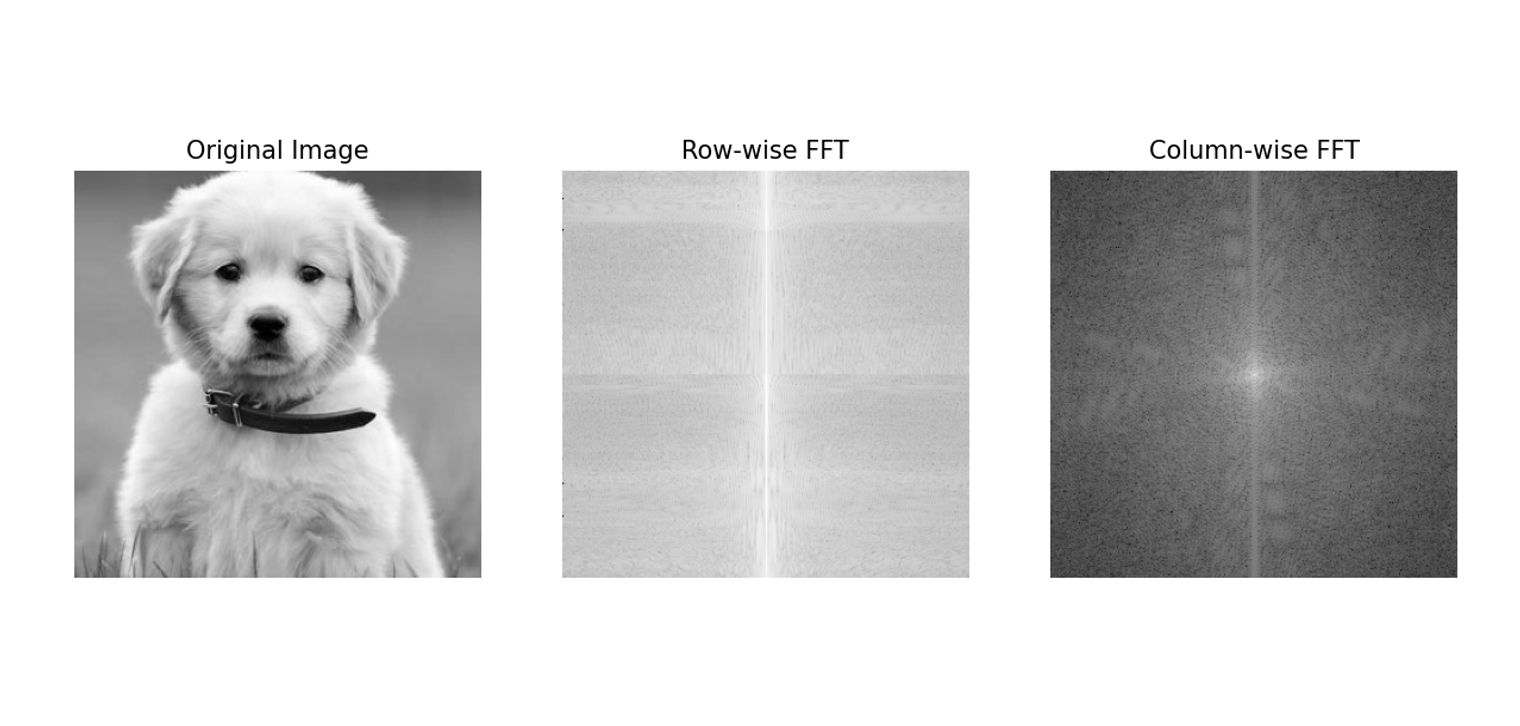
\includegraphics[width=0.75\textwidth]{ex212_output}
    \caption{After DFT\_2D() function}
    \label{ex212_output}
\end{figure}


\section{Ex 2.3 và Ex 2.4}
\subsection{Source code}
\subsubsection{filter\_frequency() function}
\begin{lstlisting}[caption={Code of filter\_frequency() function}, label={filter\_frequency()}]
def filter_frequency(orig_img, mask):
    # Fourier transform of the original image
    f_img = fft2(orig_img)

    # Shift frequency coefficients to center
    f_img_shifted = fftshift(f_img)

    # Apply mask in frequency domain
    f_img_filtered = f_img_shifted * mask

    # Shift frequency coefficients back
    f_img_filtered_shifted = ifftshift(f_img_filtered)

    # Inverse transform
    img = np.abs(ifft2(f_img_filtered_shifted))

    return f_img_filtered, img
\end{lstlisting}

\begin{itemize}
    
    \item Algorithm:
    \begin{itemize}
        \item Fourier transform of the original image (orig\_img): The original image is converted from the spatial domain to the frequency domain using the Fourier transform (fft2), creating a frequency image (f\_img).
        \item Shift frequency coefficients to center: The frequency coefficients of the image are shifted to center using the fftshift function. This is necessary to prepare for the application of the mask.
        \item Apply mask in frequency domain: Mask is applied directly to the frequency shifted image (f\_img\_shifted). This mask is pixel-mapped from the corresponding pixel on the frequency image.
        \item Backshift the frequency coefficients: After applying the mask, the frequency coefficients are shifted back to their original positions using ifftshift.
        \item Inverse transform: Finally, inverse Fourier transform (ifft2) is applied to convert the image from the frequency domain back to the spatial domain. The absolute value of the result is taken to ensure the true value.
    \end{itemize}
\end{itemize}


\subsubsection{create\_hybrid\_img() function}
\begin{lstlisting}[caption={Code of reate\_hybrid\_img() function}, label={reate\_hybrid\_img()}]
def create_hybrid_img(img1, img2, r):
    # Step 1: Fourier transform for two input images
    img1_fft = fft2(img1)
    img2_fft = fft2(img2)

    # Step 2: Shift the frequency coefficients to center using fftshift
    img1_fft_shifted = fftshift(img1_fft)
    img2_fft_shifted = fftshift(img2_fft)

    # Step 3: Create mask based on radius (r)
    rows, cols = img1.shape
    crow, ccol = rows // 2, cols // 2
    mask = np.zeros((rows, cols), dtype=np.float32)
    for i in range(rows):
        for j in range(cols):
            dist = np.sqrt((i - crow) ** 2 + (j - ccol) ** 2)
            if dist <= r:
                mask[i, j] = 1

    # Step 4: Combine frequencies of two images using mask
    img1_hybrid_fft = img1_fft_shifted * mask
    img2_hybrid_fft = img2_fft_shifted * (1 - mask)
    hybrid_img_fft = img1_hybrid_fft + img2_hybrid_fft

    # Step 5: Shift the frequency coefficients back using ifftshift
    hybrid_img_fft_shifted = ifftshift(hybrid_img_fft)

    # Step 6: Invert transform using ifft2
    hybrid_img = np.abs(ifft2(hybrid_img_fft_shifted))

    return hybrid_img
\end{lstlisting}

\begin{itemize}
    
    \item Algorithm:
    \begin{itemize}
        \item Fourier transform: Performs a Fourier transform for two input images (img1 and img2) using the fft2 function, transforming the images from the spatial domain to the frequency domain.
        \item Shift frequency coefficients: The frequency coefficients of both images are shifted to the center using fftshift.
        \item Create Mask: A mask is created based on the provided radius r. This mask is a binary array where pixels within the radius are set to 1, and pixels outside the radius are set to 0. It determines which frequencies from img1 will dominate in the hybrid image.
        \item Combine frequencies: The frequency components of both images are combined using the mask created above, ensuring that the hybrid image will have dominant frequencies from img1 within the specified radius specified, and the frequencies from img2 are outside that radius.
        \item Re-shift frequency coefficients: After combining the frequencies, the frequency coefficients of the resulting hybrid image are shifted back to their original positions using ifftshift.
        \item Inverse transform: Finally, inverse Fourier transform (ifft2) is applied to obtain hybrid images in the spatial domain. The absolute value of the inverse transform is taken to ensure the true value of the output.
    \end{itemize}
\end{itemize}



\subsection{Output}
\subsubsection{Result after executing filter\_frequency() function}
\begin{itemize}
    \item Photos obtained:
\end{itemize}

\begin{figure}[H]
    \centering
    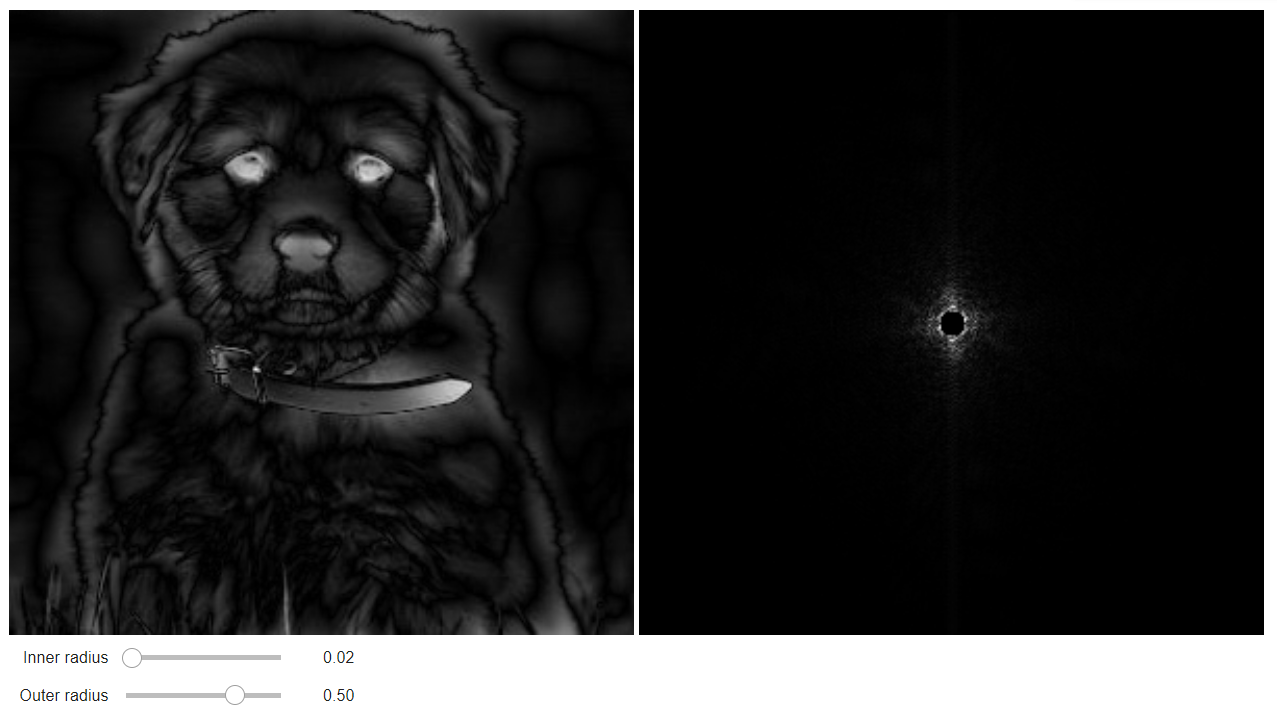
\includegraphics[width=0.75\textwidth]{ex23_output}
    \caption{After filter\_frequency() function}
    \label{ex23_output}
\end{figure}


\subsubsection{Result after executing create\_hybrid\_img() function}
\begin{itemize}
    \item Photos obtained:
\end{itemize}

\begin{figure}[H]
    \centering
    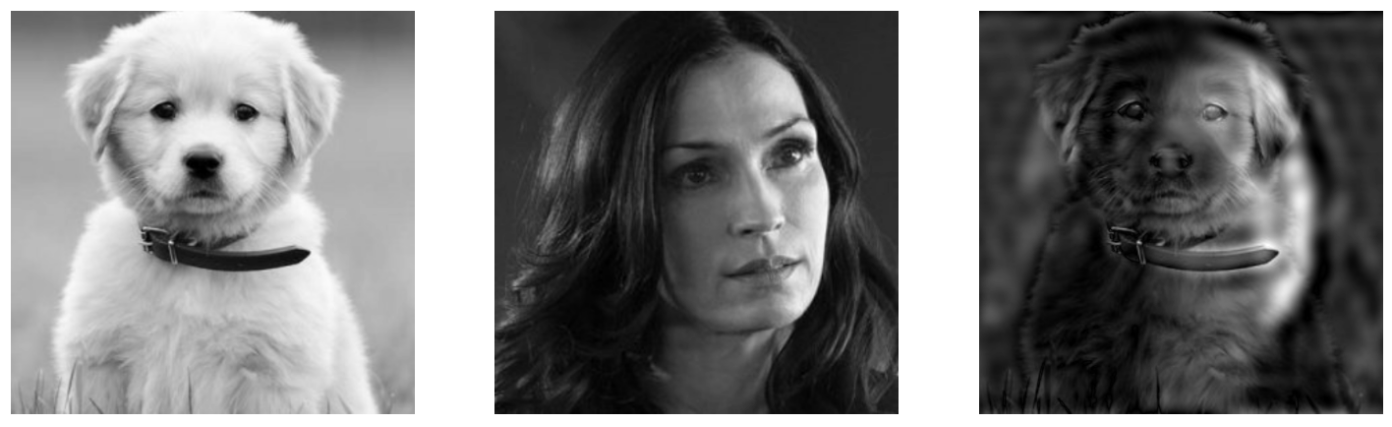
\includegraphics[width=0.75\textwidth]{ex24_output}
    \caption{After create\_hybrid\_img() function}
    \label{ex24_output}
\end{figure}



\end{document}
